% !TeX root = ../main.tex

\chapter{实验结果与分析}
实验的主要目的是为了解决以下的问题:

(1) 学到的角色是否能够动态地变化,并且这种变化是为了适应环境?(章节~\ref{sec:dynamic-role})

(2) 本框架能否促进子任务的分化、专业化?即拥有相似任务的智能体在角色空间有相似的角色表征,但是有不同的子任务的智能体有不同的角色,并且这个角色在角色空间相差很远。(章节~\ref{sec:role-evolution})

(3) 这样的子任务分化能否提高多智能体强化学习的性能?(章节~\ref{sec:baseline-ablation})

(4) 角色在训练的过程中是怎样演化的?以及这种演化对性能的影响是怎样?(章节~\ref{sec:role-evolution})

本相关实验的视频能在网站上看到\footnote{\url{https://sites.google.com/view/romarl/}}。项目的代码已公开\footnote{\url{https://github.com/drdh/pymarl}}

\section{基准实验和消融实验}\label{sec:baseline-ablation}

\begin{table}[htb]
    \centering\small
    \caption{基准实验和消融实验算法}
    \label{tab:baselines}
    \begin{tabular}{cll}
      \toprule
        & 算法   & 描述                         \\
      \midrule
          & IQL   & Independent Q-learning \\
          & COMA  & Foerster et~al.~\cite{foerster2018counterfactual} \\
      相关  & QMIX  & Rashid et~al.~\cite{rashid2018qmix} \\
      算法  & QTRAN & Son et~al.~\cite{son2019qtran} \\
          & MAVEN & Mahajan et~al.~\cite{mahajan2019maven} \\
      \midrule 
             & ROMA-RAW & 无损失函数$\mathcal{L}_I$和$\mathcal{L}_D$ \\
      消融-A    & QMIX-NPS & 每个智能体都有单独的局部效用网络的QMIX \\
            & QMIX-LAR & 带有和ROMA相当数量参数的QMIX \\
       \midrule
            & $\mathcal{L}_{TD}$ & 仅有TD损失函数,同ROMA-RAW \\
      消融-B & $\mathcal{L}_{TD}+\mathcal{L}_I$ & 没有$\mathcal{L}_D$的ROMA \\
            & $\mathcal{L}_{TD}+\mathcal{L}_D$ & 没有$\mathcal{L}_I$的ROMA \\
      \bottomrule
    \end{tabular}
  \end{table}

  本实验采用的基准实验和消融实验如表~\ref{tab:baselines}所示,ROMA(Role-Oriented MARL)代指本项目算法。其中,相关算法(见图~\ref{fig:performance-baselines})是为了明确比较本算法和其他已有的算法的性能,可以看到本算法有相当优异的性能;消融-A实验中(见图~\ref{fig:performance-ablations-A}),ROMA-RAW是为了明确上一章所介绍的损失函数的有效性;QMIX-NPS是为了说明独立的效用函数并不能达到本项目算法的性能;QMIX-LAR是为了说明更多的参数不是本算法性能提升的主要原因;消融-B实验见图~\ref{fig:performance-ablations-B})是为了明确各个损失函数对性能的影响。

  测试的环境是星际争霸2微操作基准(SAMC~\cite{samvelyan2019starcraft}). 这个环境包括各种各样的地图,这些地图被分类成简单、难、很难几个级别。上面选取的环境都是难或者很难。为了评估准确,所有的实验都是使用了5的随机种子,结果的曲线是带有$95\%$的置信区间的。

\begin{figure*}
    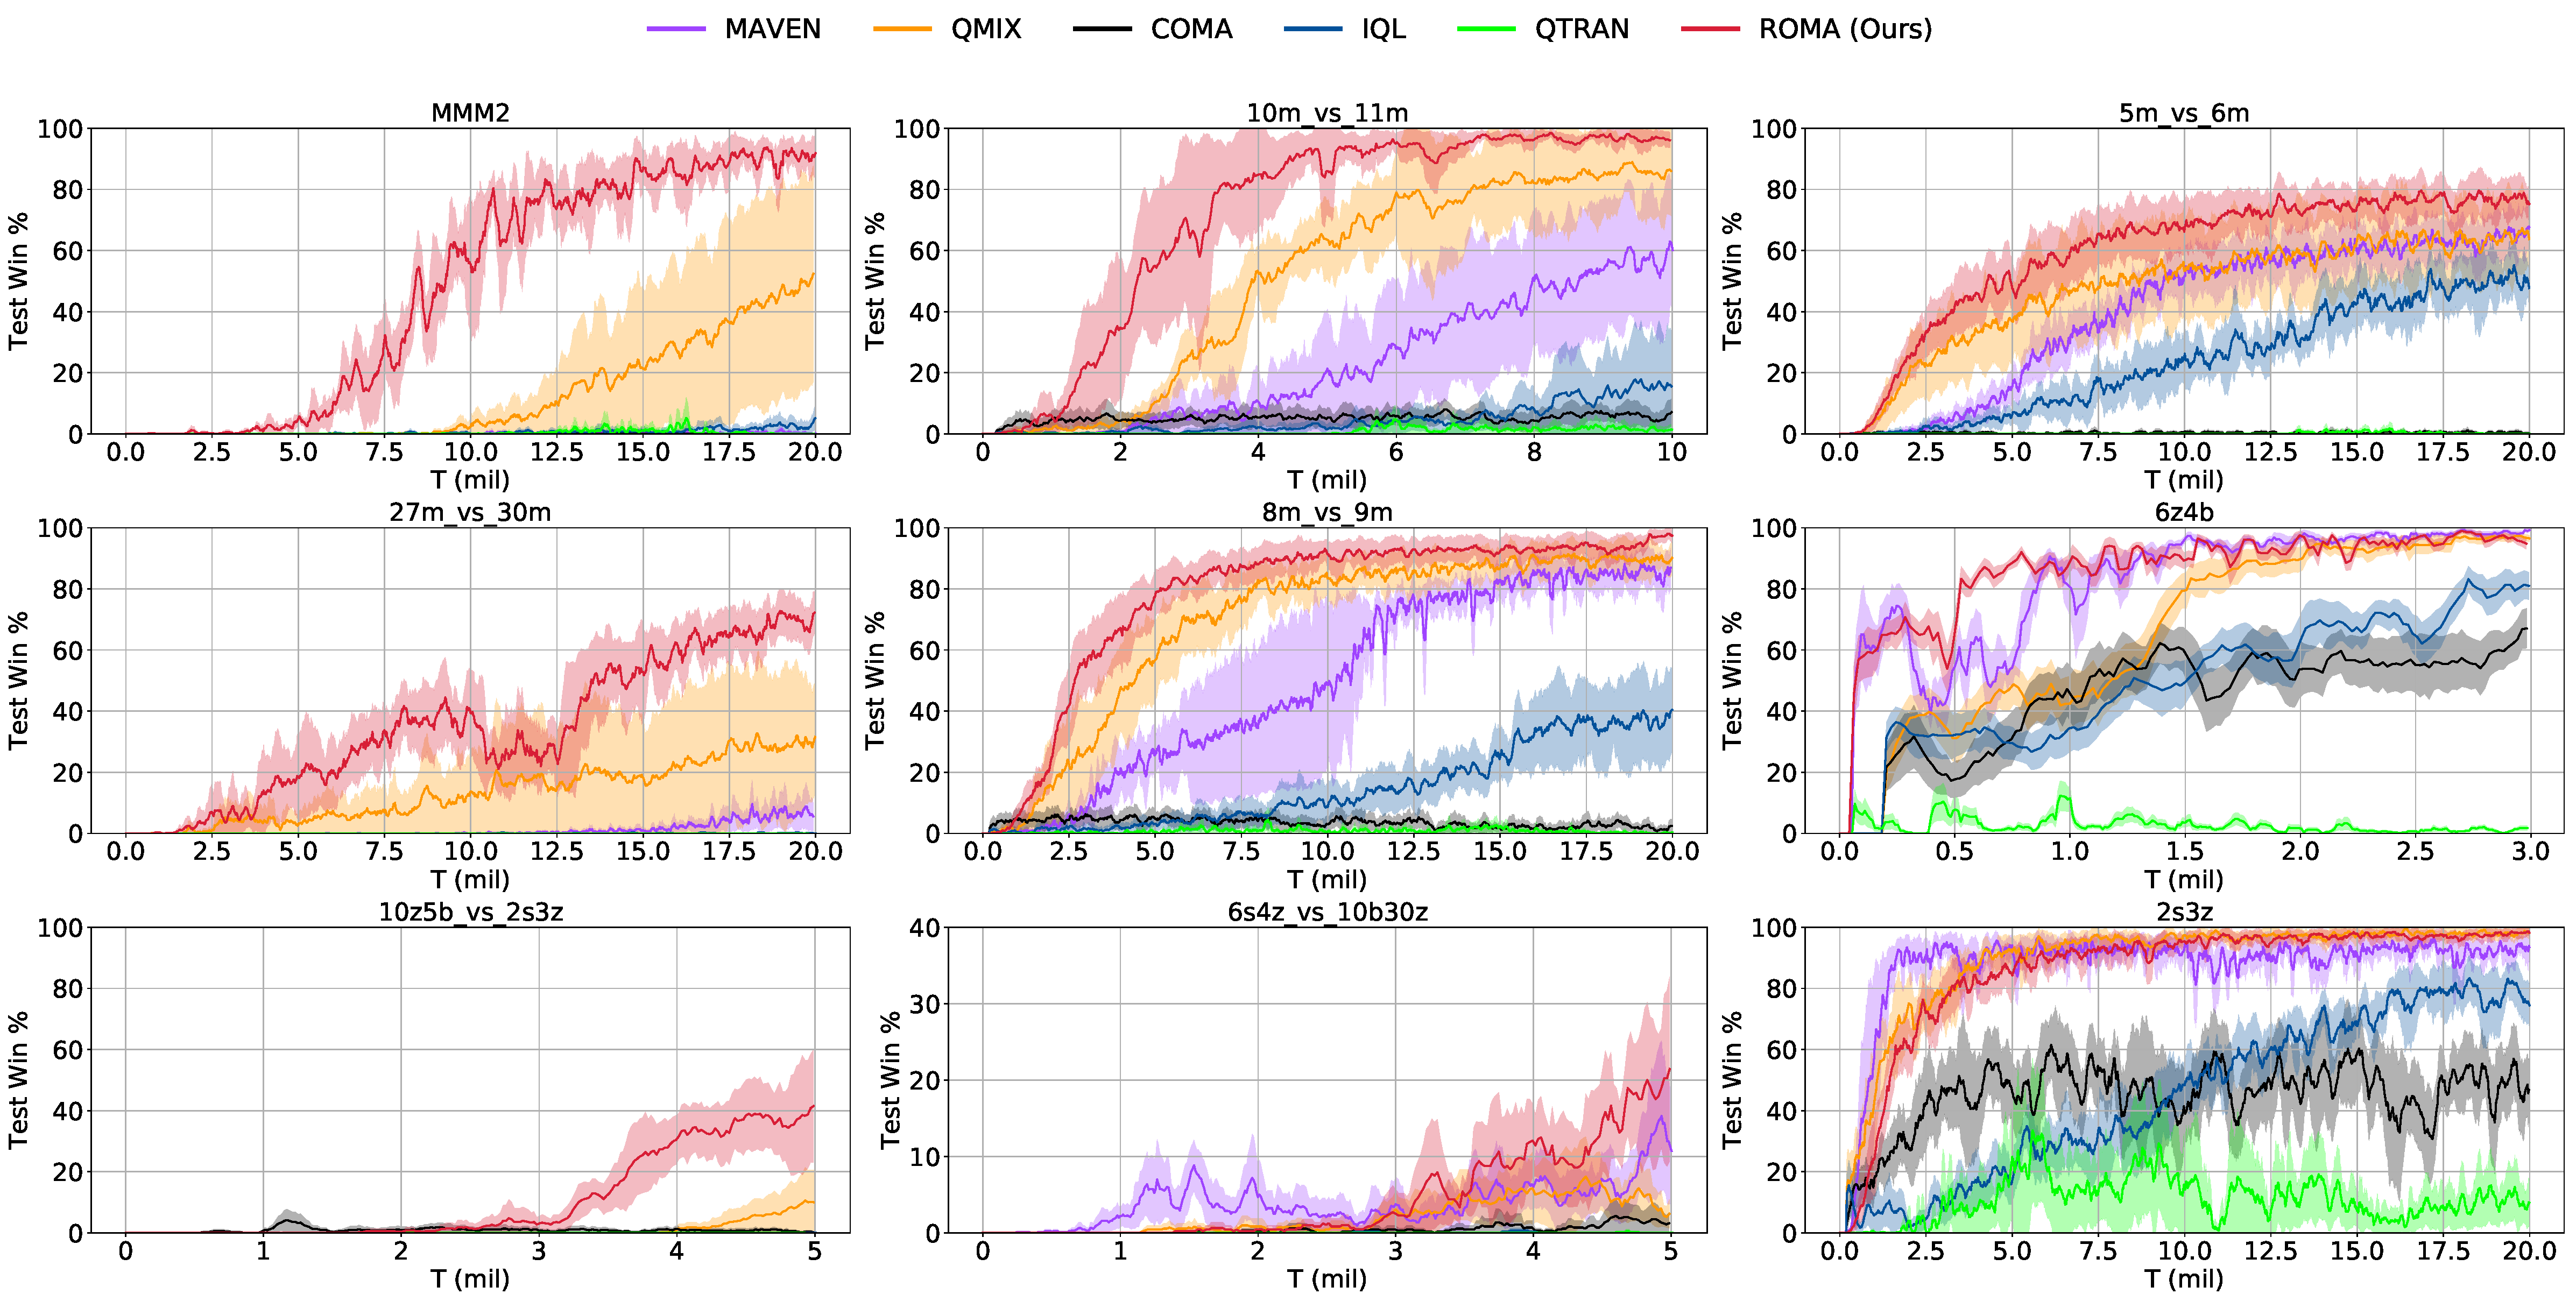
\includegraphics[width=\linewidth]{figures/learning-curve/learning_curve.pdf}
    \caption{ROMA与相关算法的性能对比}\label{fig:performance-baselines}
\end{figure*}

\begin{figure*}
    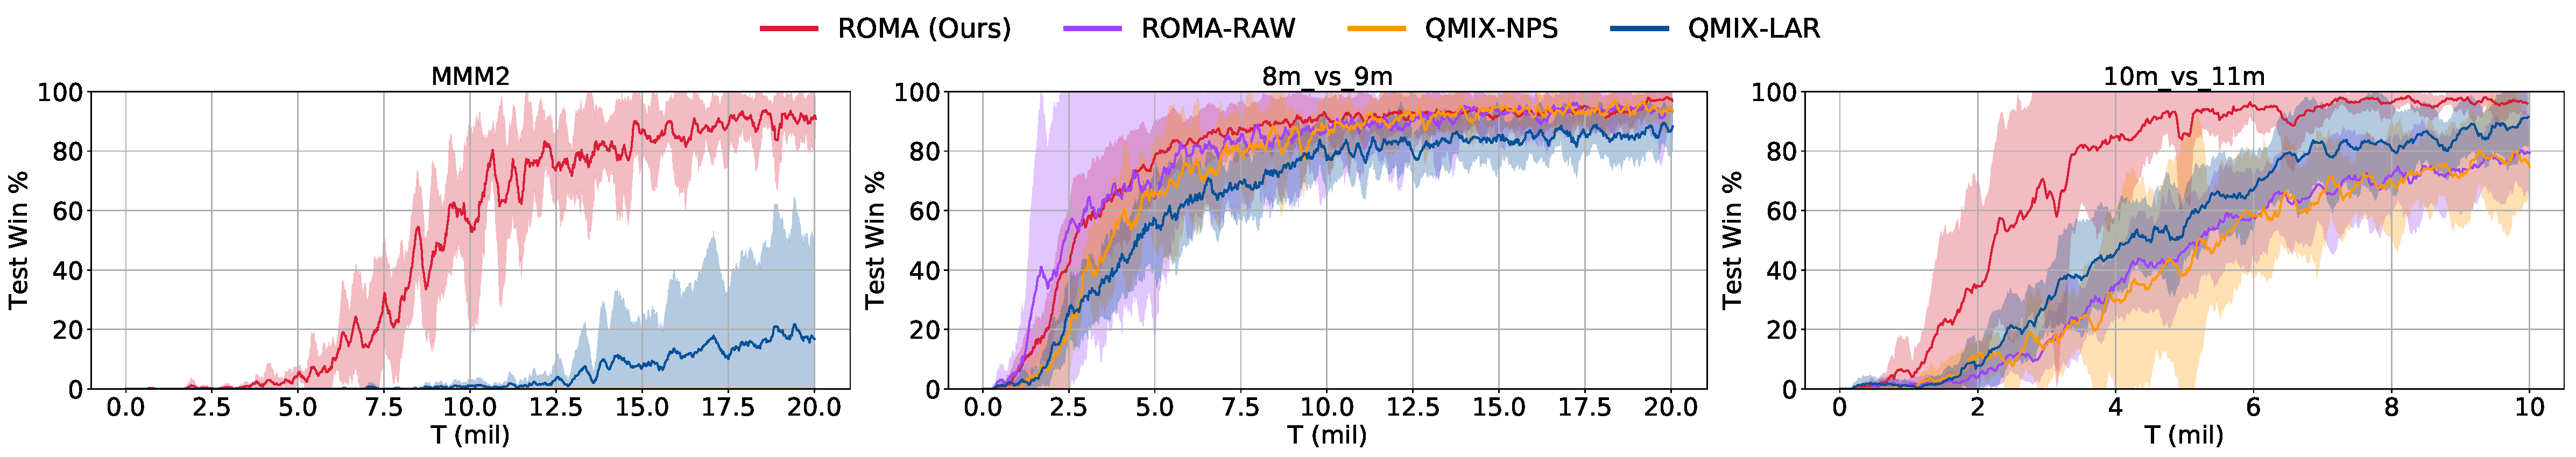
\includegraphics[width=\linewidth]{figures/learning-curve/ablation-A.pdf}
    \caption{消融实验-A}\label{fig:performance-ablations-A}
\end{figure*}

\begin{figure*}
    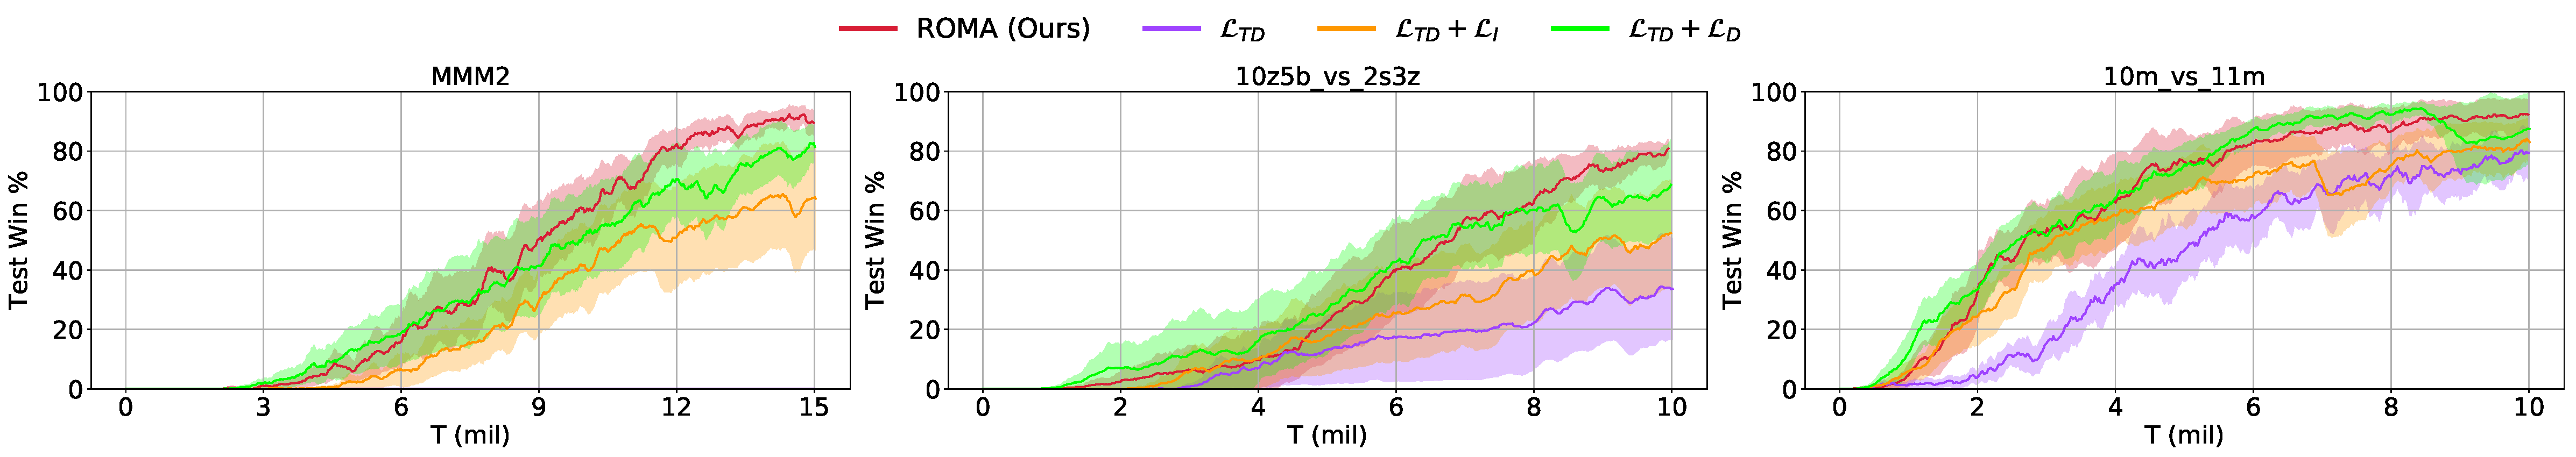
\includegraphics[width=\linewidth]{figures/learning-curve/ablation-B.pdf}
    \caption{消融实验-B}\label{fig:performance-ablations-B}
\end{figure*}
  
\section{角色的动态变化}\label{sec:dynamic-role}

为了回答角色是否是为了使用环境动态变化的,这里展示几张由本算法执行的截图,使用的环境是星际争霸2微操作环境(SMAC), 选用的地图是$\mathtt{10m\_vs\_11m}$, 在这个环境里,操控10个Marines对抗11个敌对Marines. 

\begin{figure*}
    \centering
    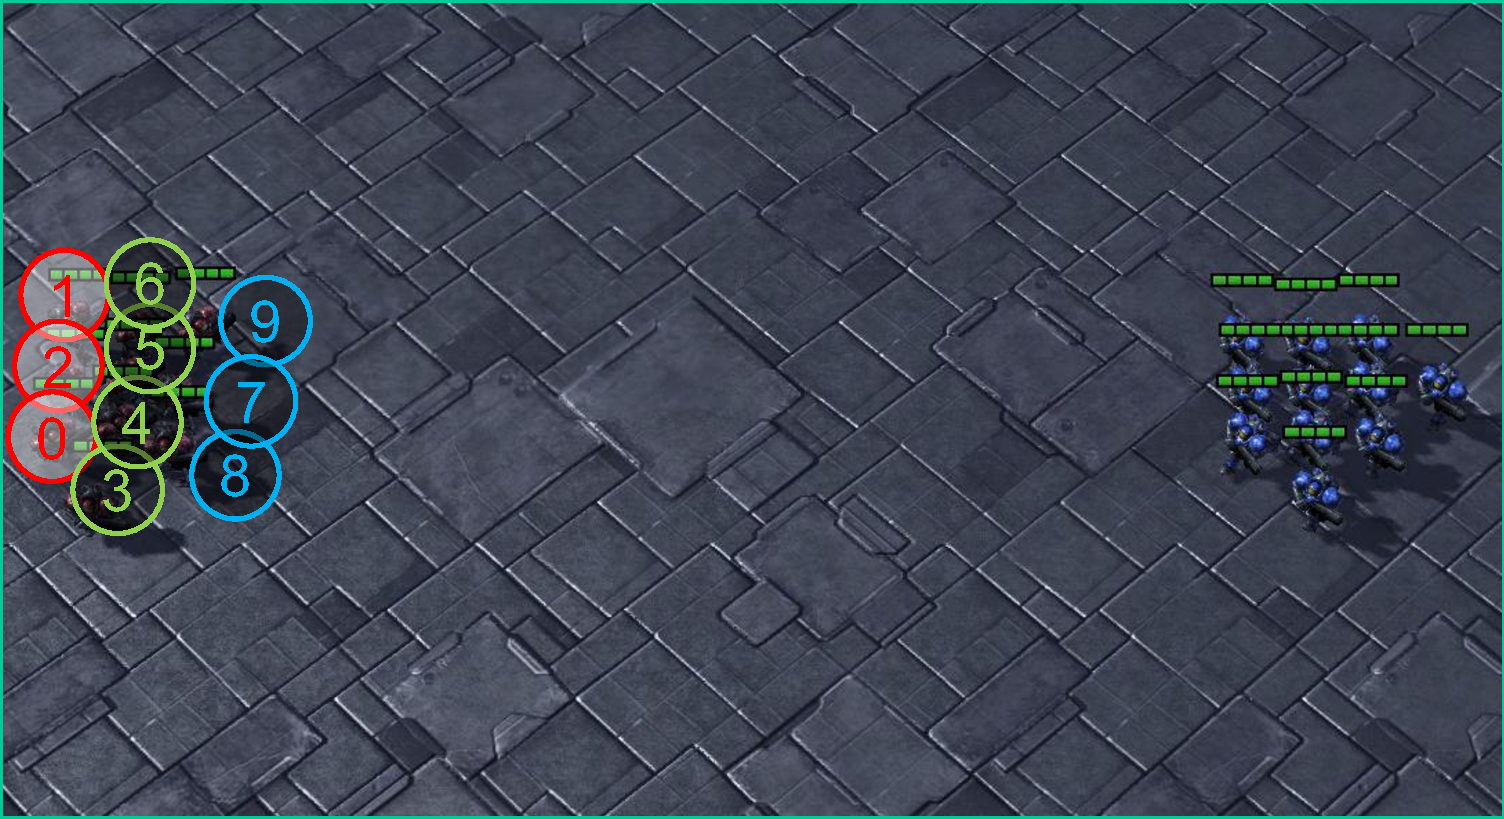
\includegraphics[height=0.24\linewidth]{figures/dynamic/10m_vs_11m-g1.pdf}\hfill
    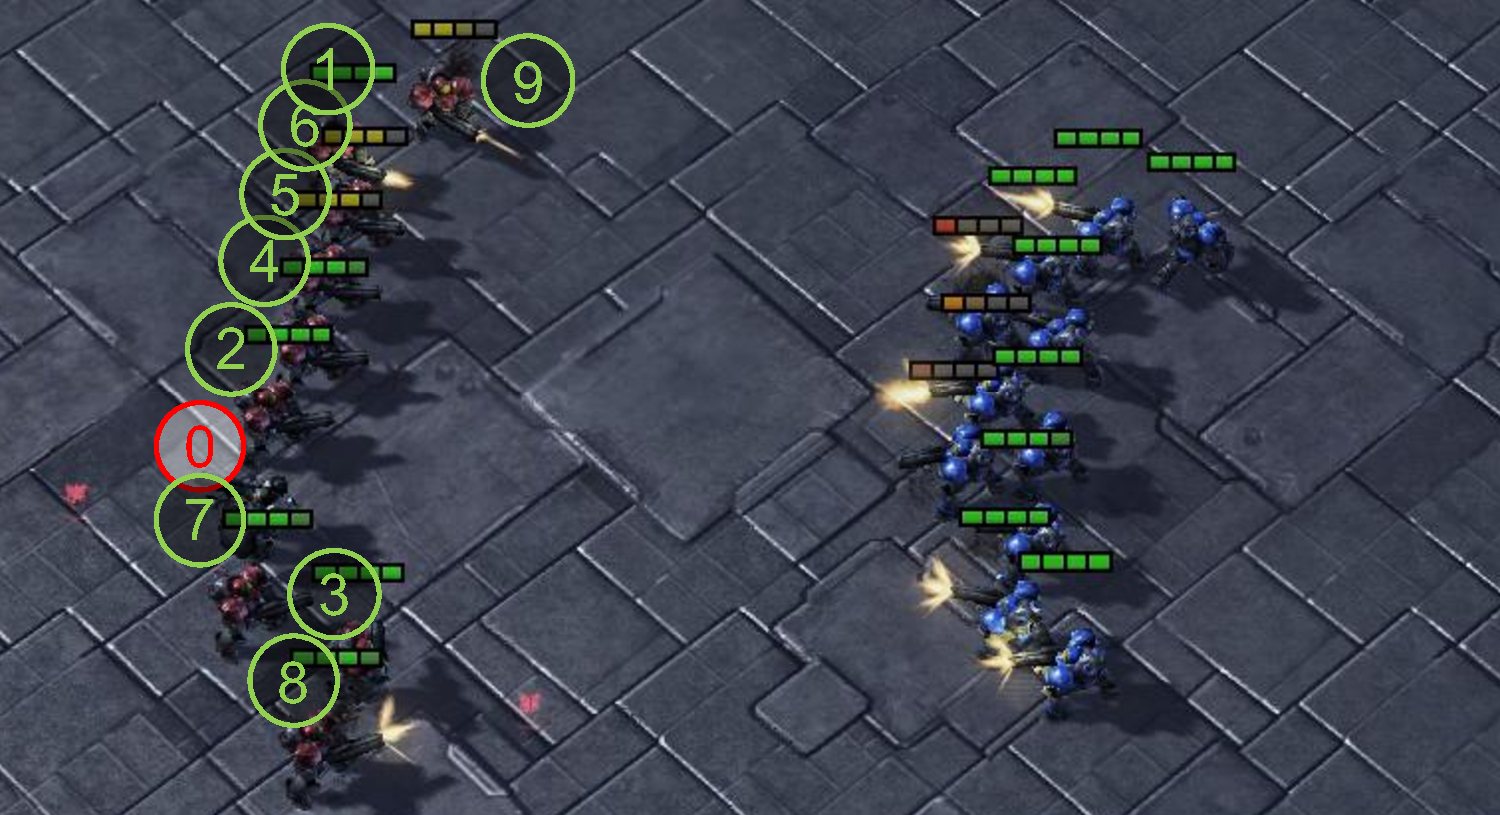
\includegraphics[height=0.24\linewidth]{figures/dynamic/10m_vs_11m-g2.pdf}\\
    \subfigure[$t$=$1$, 角色的特征是智能体的位置]{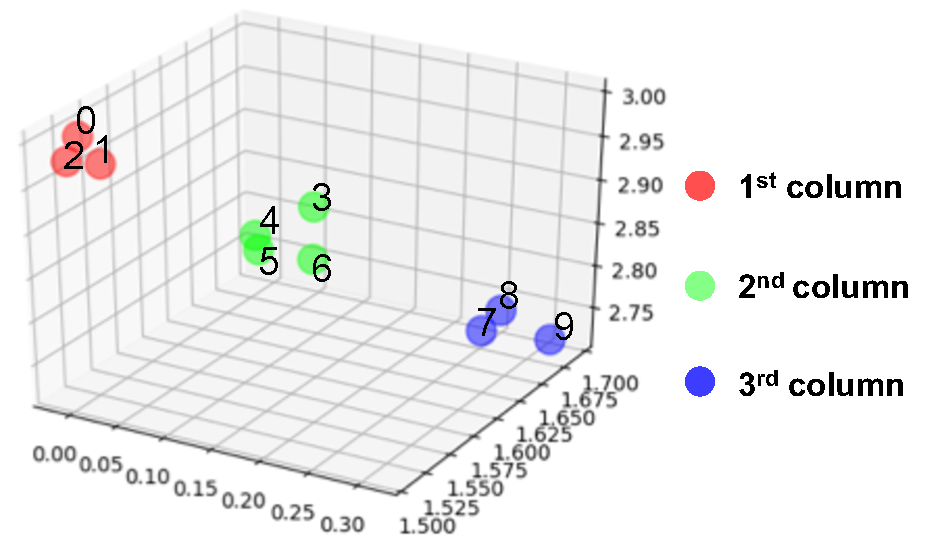
\includegraphics[width=0.48\linewidth]{figures/dynamic/10m_vs_11m-r1.pdf}}\hfill
    \subfigure[$t$=$8$, 角色的特征是智能体的血量]{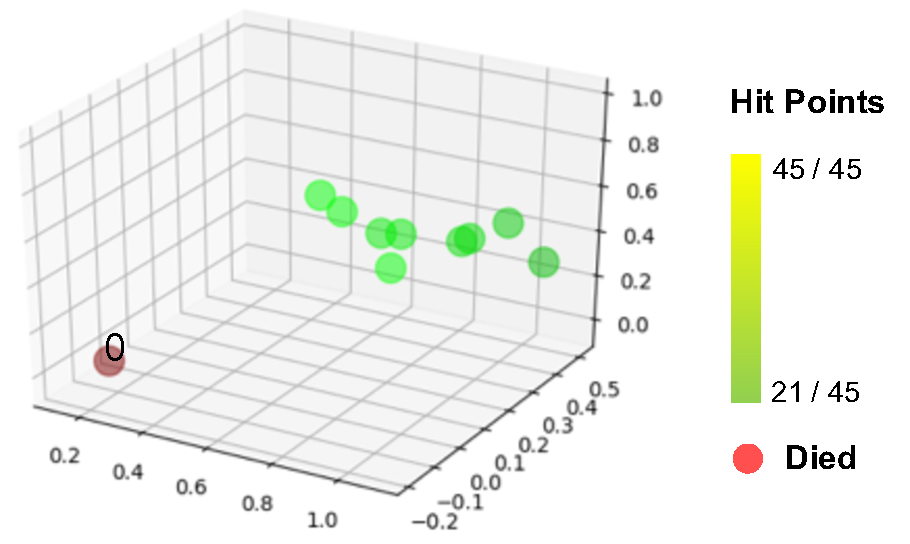
\includegraphics[width=0.48\linewidth]{figures/dynamic/10m_vs_11m-r2.pdf}}\\

    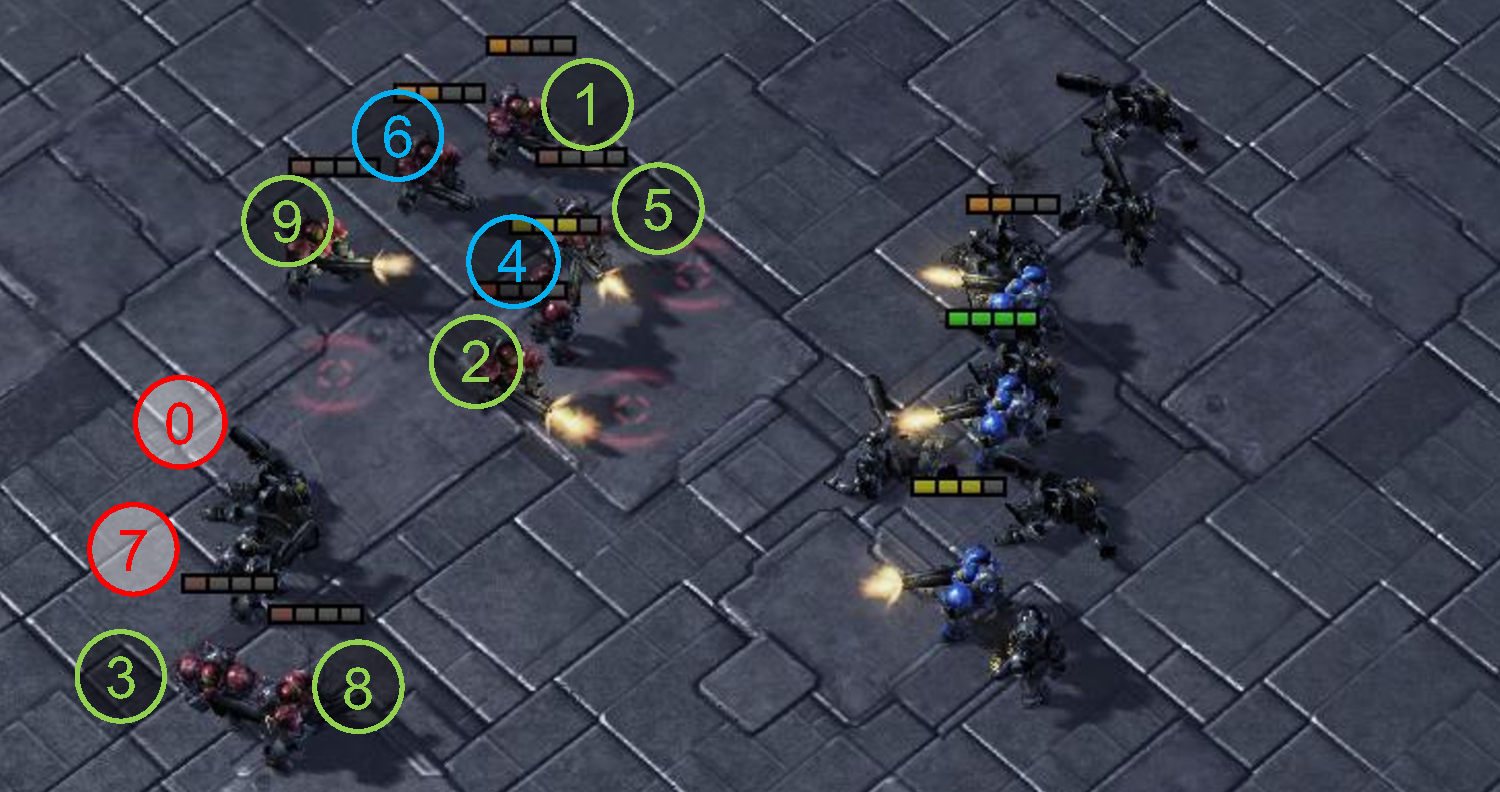
\includegraphics[height=0.24\linewidth]{figures/dynamic/10m_vs_11m-g3.pdf}\hfill
    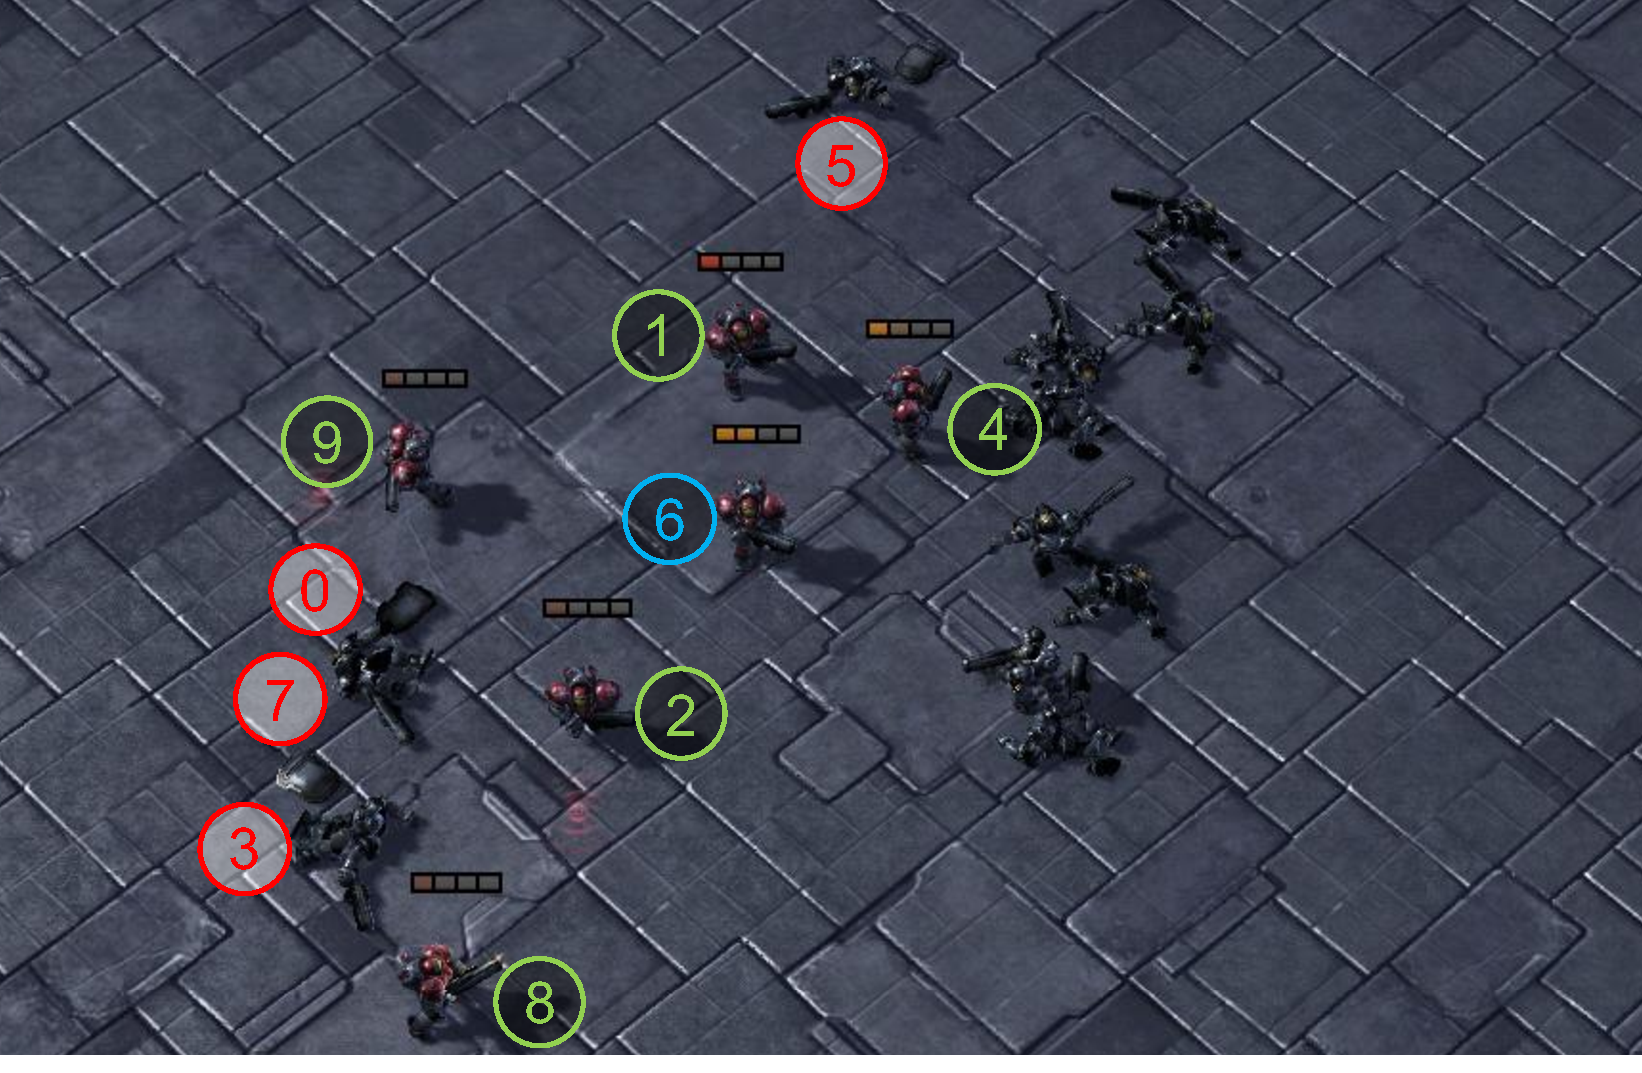
\includegraphics[height=0.24\linewidth]{figures/dynamic/10m_vs_11m-g4.pdf}\\ 
    \subfigure[$t$=$19$, 角色的特征是智能体是否存活及血量]{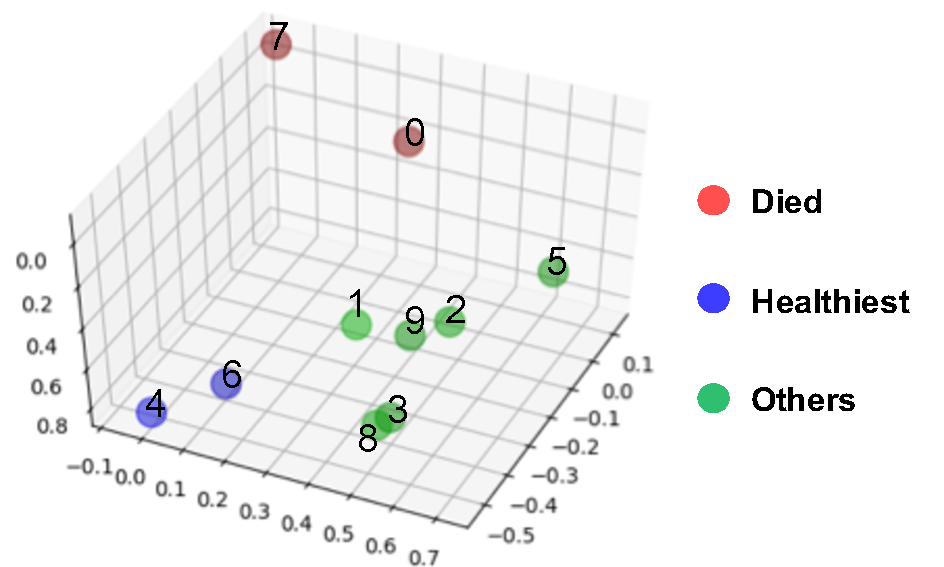
\includegraphics[width=0.48\linewidth]{figures/dynamic/10m_vs_11m-r3.pdf}}\hfill
    \subfigure[$t$=$27$, 角色的特征是智能体是否存活及血量]{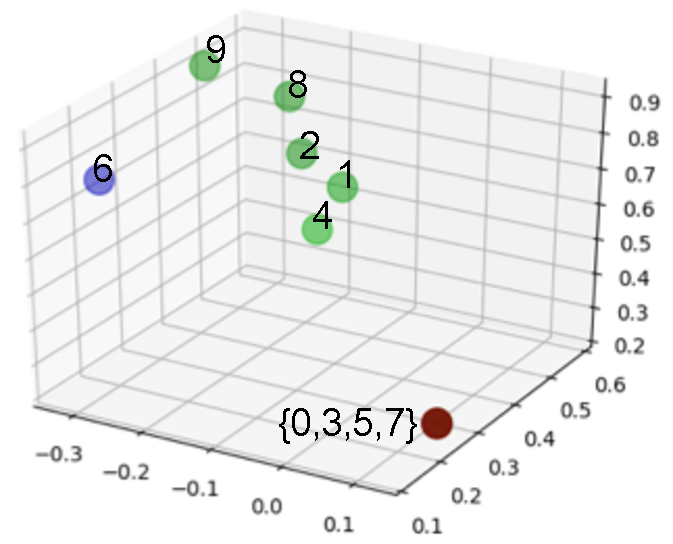
\includegraphics[width=0.32\linewidth]{figures/dynamic/10m_vs_11m-r4.pdf}}
    \caption{在一局里角色的动态变化}\label{fig:dynamic_role-10m_vs_11m}
\end{figure*}
正如图~\ref{fig:dynamic_role-10m_vs_11m}所示,尽管观测里包含很多的信息,比如智能体的位置、血量、护盾值、同盟信息、敌人信息等等,但是角色编码器还是学会了集中注意力到部分关键的信息,并且这种注意力会随着环境的改变,动态地变化,这就是所谓的角色的动态变化。

具体来说,在刚开始$t$=$1$的时候,智能体们需要组织成为一个凹面的弧形,这样能最大化它们对敌人的射击范围,使得每个智能体都能射击到敌人最前面的那一行。可以从角色空间看到的是智能体角色的排布是根据它们的相对位置,如此根据这样的特化的策略能更快地形成上面提到的弧形站位。在战役的中间,一个很有用的策略是保护受伤严重的智能体,让它们后撤,这样能最大限度地保存战力,消灭敌人。可以从图中看到,在$t$=$8$, $19$, $27$的时候,智能体的角色决定于它自己的血量,血量高的智能体角色和其他智能体的角色相距很远。这样的表征会导致不同的策略:也就是血量高的智能体会向前移,吸引更多的火力,而其他的血量低的会后撤,从后方攻击。与此同时,也能发现同样的角色会因为位置相近而聚集在一起,比如智能体$3$和$8$在$t$=$19$的时候就聚在一起了。对应的策略是拥有不同角色的智能体会不断变换地吸引火力。除此之外,也能看到死亡的智能体会聚集在一起,并且数量不断增多,本质上来说,死亡是血量为$0$的极端情况。

这个结果就说明,本算法能够学到动态的角色,并且角色会依据自己观测到的子任务(比如前进、后撤)自动聚集,这一点也和上一章提出的目标函数的目的一致。

\section{角色的表征分析}\label{sec:role-representation}
\begin{figure*}
  \centering
  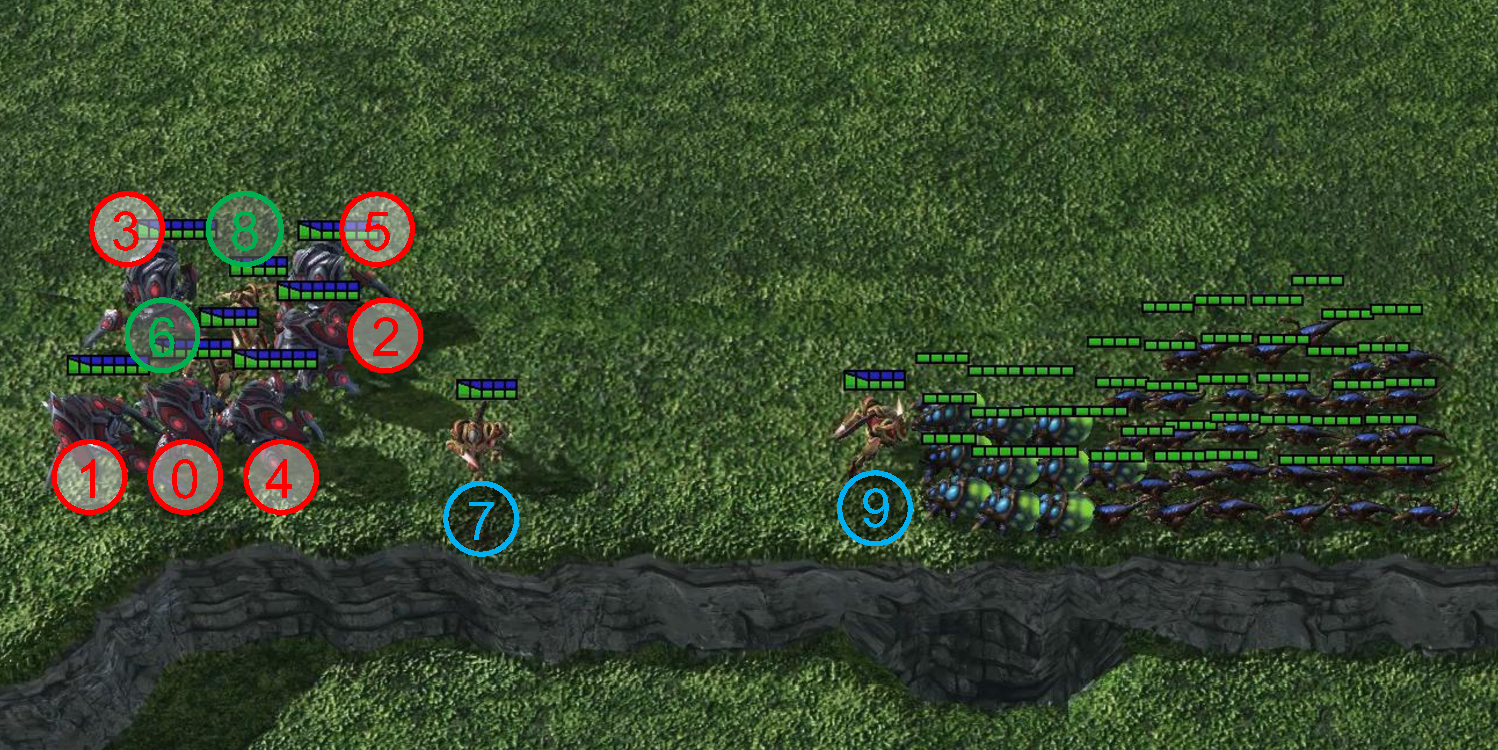
\includegraphics[width=0.32\linewidth]{figures/various-roles/various_roles-g1.pdf}\hfill
  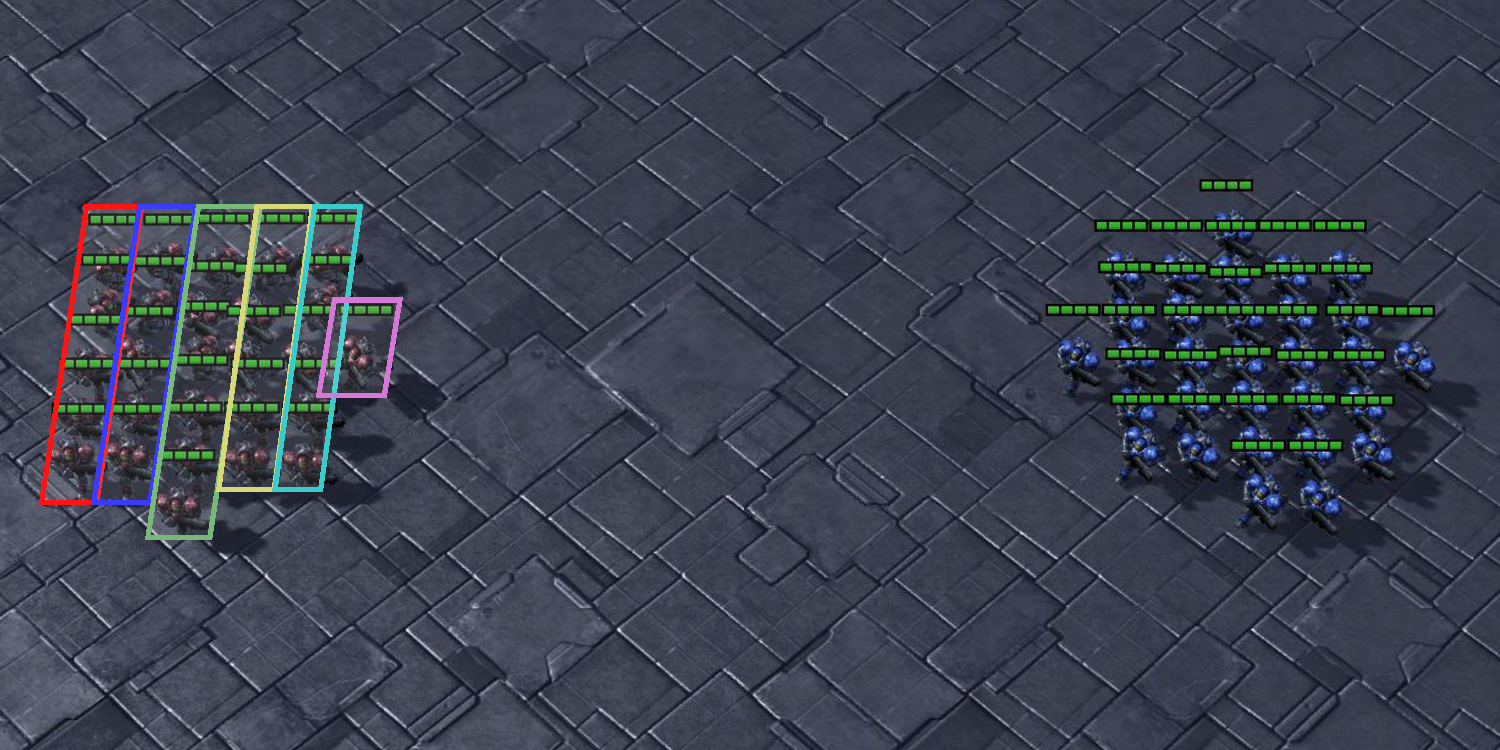
\includegraphics[width=0.32\linewidth]{figures/various-roles/various_roles-g2.pdf}\hfill
  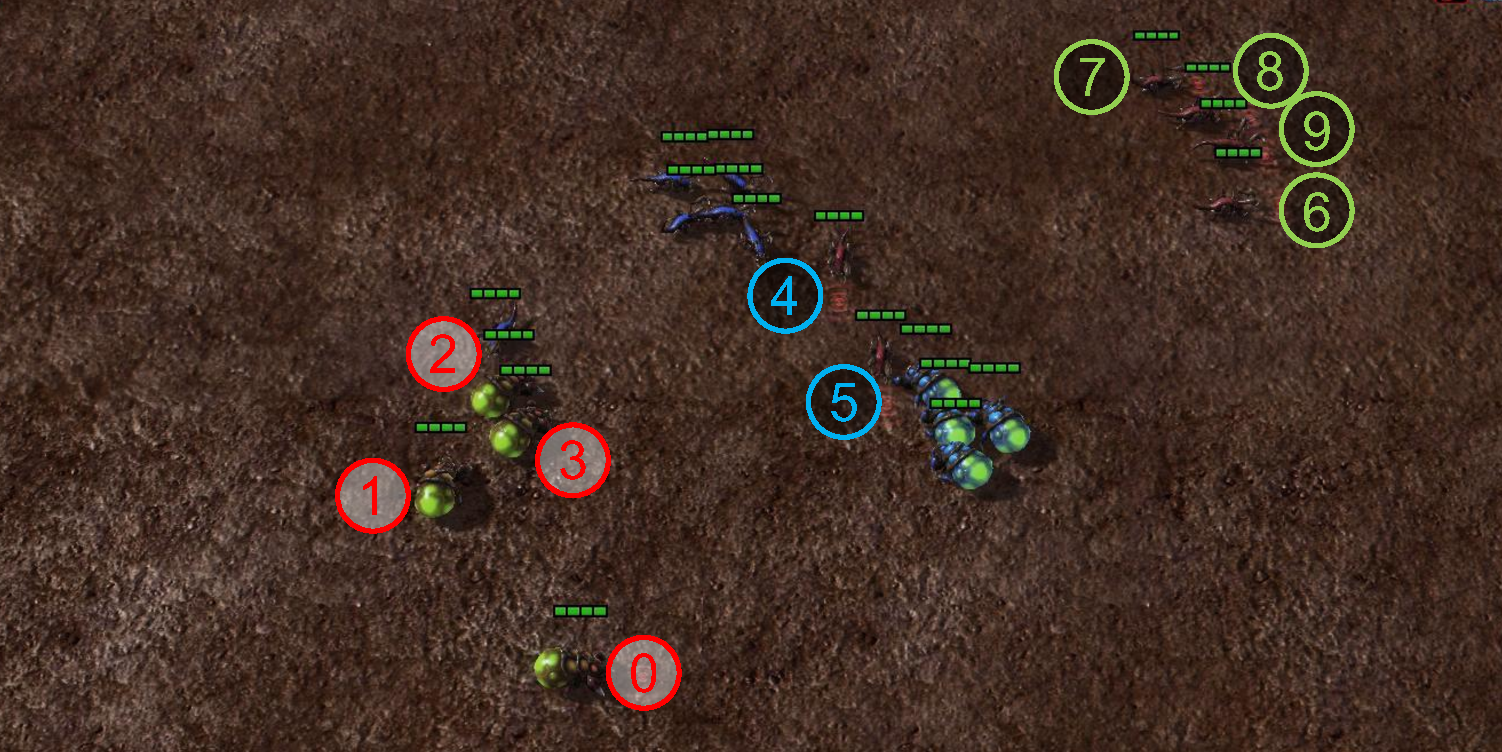
\includegraphics[width=0.32\linewidth]{figures/various-roles/various_roles-g3.pdf}
  \subfigure[策略:牺牲Zealots 9和7来消除Banelings的爆炸伤害。]{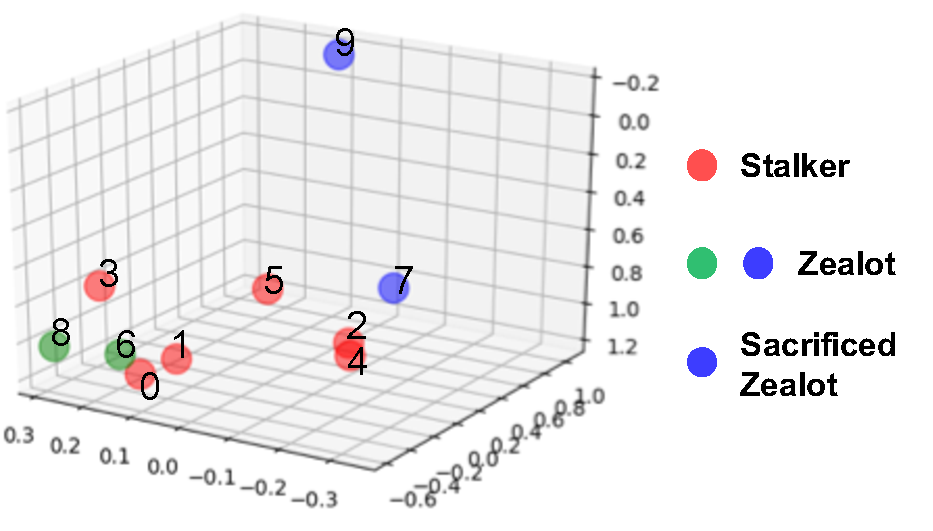
\includegraphics[width=0.32\linewidth]{figures/various-roles/various_roles-r1.pdf}\label{fig:various_roles-6s4z_vs_10b30z}}\hfill
  \subfigure[策略:快速形成一个凹型的站位。]{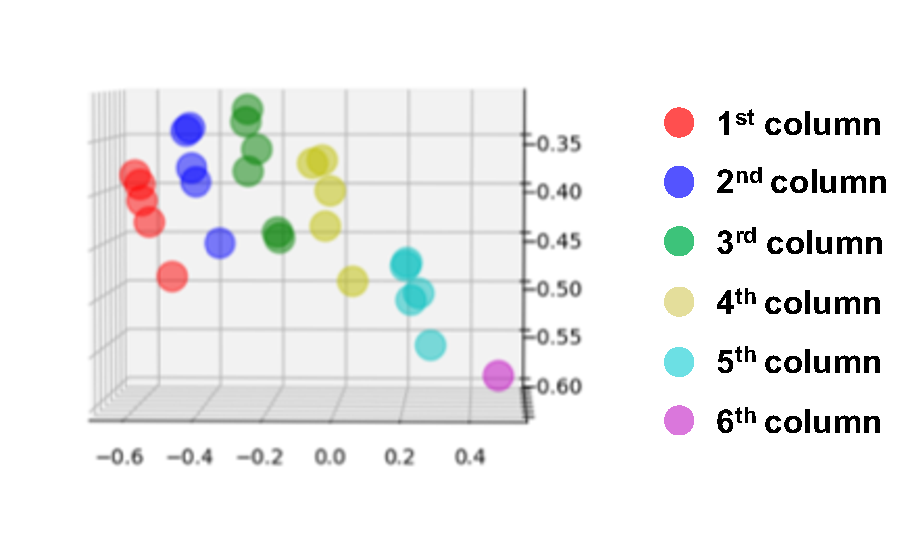
\includegraphics[width=0.32\linewidth]{figures/various-roles/various_roles-r2.pdf}\label{fig:various_roles-27m_vs_30m}}\hfill
  \subfigure[策略:绿色的Zerglings躲起来,然后Banelings用爆炸消灭大部分的敌人。]{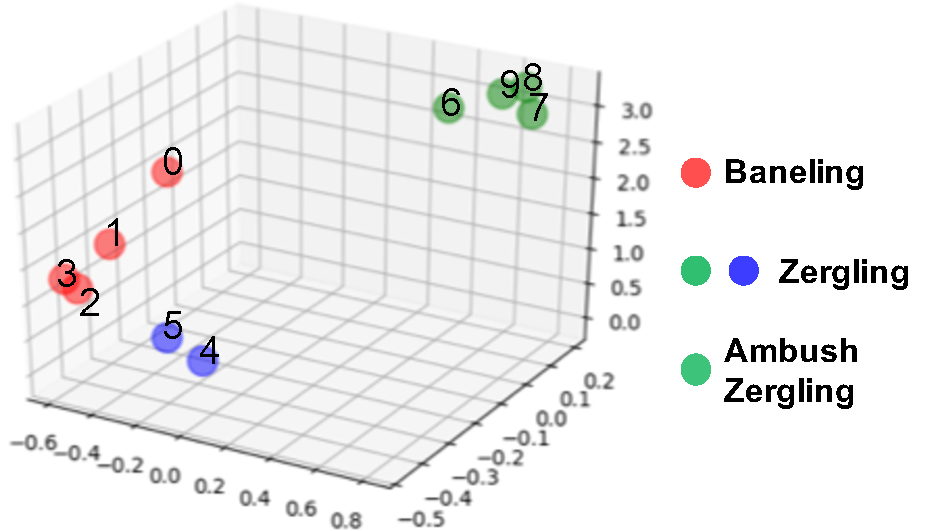
\includegraphics[width=0.32\linewidth]{figures/various-roles/various_roles-r3.pdf}\label{fig:various_roles-6z4b}}
  \caption{角色的表征}\label{fig:various_roles}
  \note{地图$\mathtt{6s4z\_vs\_10b30z}$, $\mathtt{27m\_vs\_30m}$,和$\mathtt{6z4b}$学到的角色表征 (展示的是角色$\bm{\mu}_{\rho_i}$的均值,没有使用任何的降维)}
\end{figure*}

为了解释本算法的有效性,用图~\ref{fig:various_roles}来展示角色在角色空间的表征。注意到角色表示的是自动发现的胜利策略在隐层空间的表征,下面逐一说明。

在地图$\mathtt{6s4z\_vs\_10b30z}$中,见图~\ref{fig:various_roles-6s4z_vs_10b30z}, 本算法学会了牺牲Zealots 9和7来杀死所有的敌对Banelings(爆炸的Banelings自己也会死)。具体来说,Zealots 9和7会一个接着一个地向前,然后和敌人同归于尽,但是其他智能体会远离,等待直到所有的Banelings爆炸结束。图~\ref{fig:various_roles-6s4z_vs_10b30z}就是完成第一个子任务时,9号智能体牺牲时的角色表征,可以看到它的角色和其他的相距很远,这就是意味着9的策略和其他的非常不一样,从具体的回放截图也可以证实这一点。

对于地图$\mathtt{27m\_vs\_30m}$, 胜利策略是在战斗开始之初,交火之前,快速形成一个凹型的站位,图~\ref{fig:various_roles-27m_vs_30m}正是诠释了这一点,这里展示的是$t$=$1$的时刻的角色表征,智能体们正准备形成攻击站位。从角色空间也可以看到角色按照的是智能体的相对位置在聚集,这样的不同的表征会导致不同的移动策略,继而能迅速形成凹型站位,并且不发生冲突。

对于地图$\mathtt{6z4b}$, 胜利策略是Zerglings 4和5以及Banelings杀掉其他大部分的敌人,这里是利用Banelings的爆炸。同时,Zerglings 6-9会躲远,直到爆炸结束,然后再去杀掉剩下来的敌人。图~\ref{fig:various_roles-6z4b}显示的是在爆炸之前的角色表征,可以看到角色正是按照发现的子任务在聚集。

通过这些结果的证实,可以得出结论的是,本算法会自动地分解任务,并且能学到足够通用的角色,每个角色承担这样一个子任务。

\section{角色的演化与涌现}\label{sec:role-evolution}
到现在已经展示了学到的角色的表征和算法的性能,但是角色和算法的性能的关系仍然不明确。为了弥补这个,这里在训练过程中可视化角色的涌现和演化,使用两个地图,一个是有不同智能体的异质环境$\mathtt{MMM2}$, 另一个是智能体都相同的同质环境$\mathtt{10m\_vs\_11m}$.下面分别叙述。

\subsection{异质环境中角色的演化与涌现}
\begin{figure*}
  \centering
  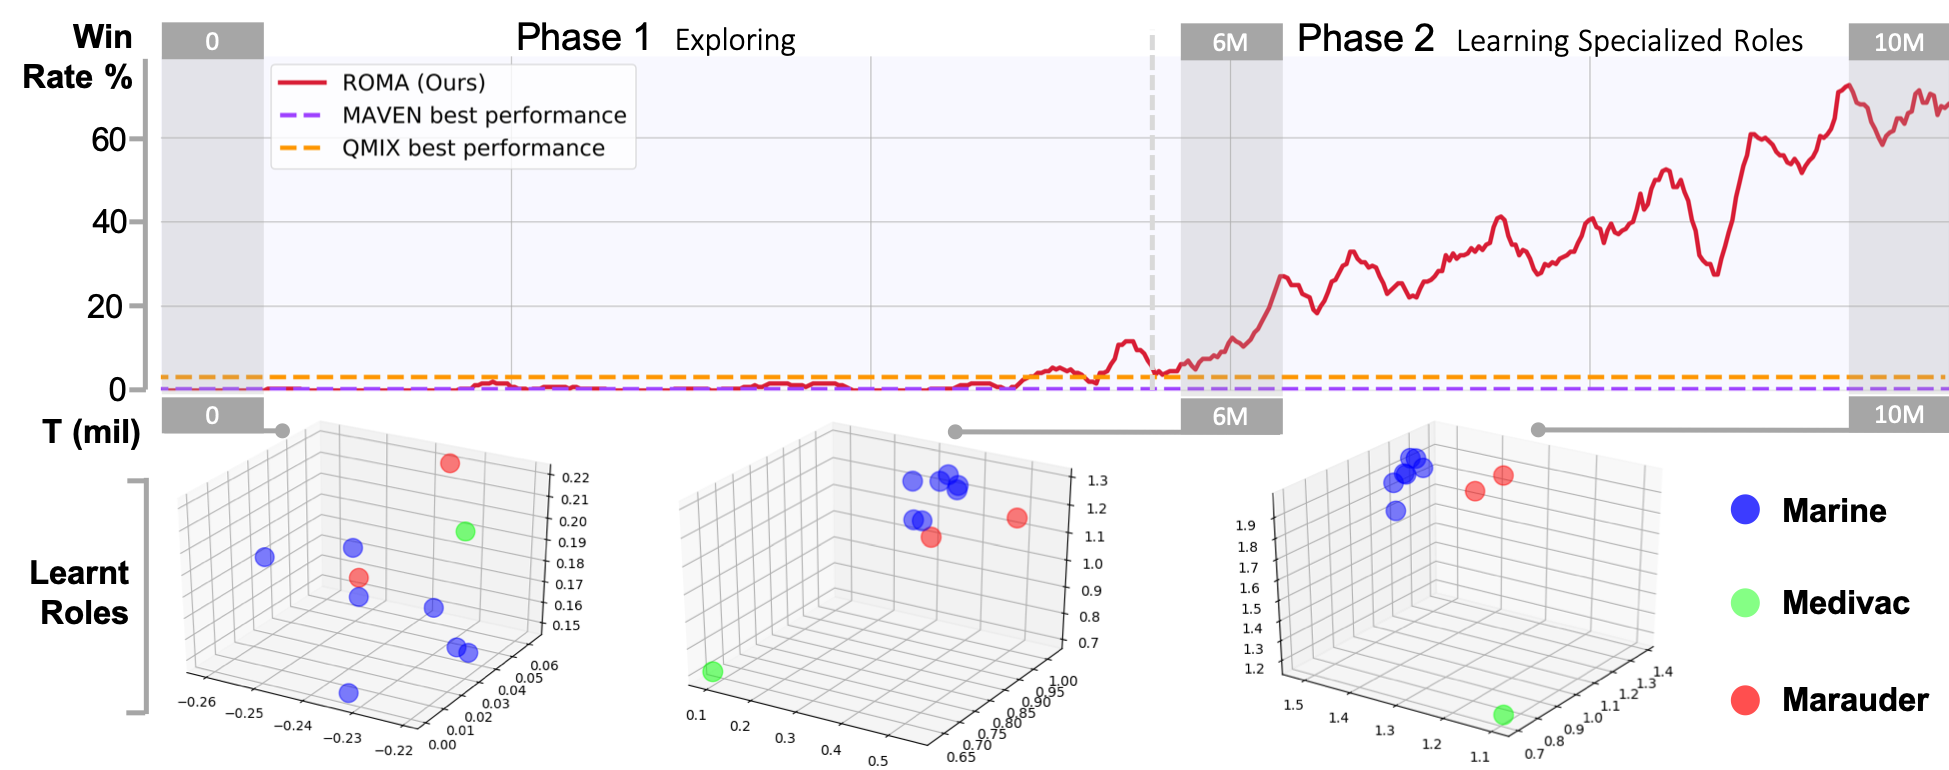
\includegraphics[width=\linewidth]{figures/evolution/evolution_MMM2.png}
  \caption{角色在$\mathtt{MMM2}$中的演化与涌现}
  \label{fig:role_evolution-heter}
  \note{展示的是$t$=$1$的角色分布的$\bm{\mu}_{\rho_i}$的均值,无任何降维。}
\end{figure*}

$\mathtt{MMM2}$环境我方智能体是1 Medivac, 2 Marauders, 和 7 Marines, 敌方智能体是1 Medivac, 3 Marauders, 和 8 Marines. 总共有三种智能体,其中,Medivac是最特殊的,因为它能够治愈其他的智能体。

在图~\ref{fig:role_evolution-heter}中,展示了本算法的其中一个训练曲线(红色),以及在每局第一步的角色表征,这里抽取三个关键的训练节点来展示角色。

刚开始的时候($T$=$0$), 角色是随机的,智能体在探索环境,学习基本的环境模型和任务结构。

在$T$=$6$M的时候,逐渐学到Medivac的任务和其他的智能体完全不一样,相应地,它的角色也和其他的智能体的角色相差很远,学习到这种行为上的区别让游戏开始逐渐出现胜局。

慢慢地,又学习到Marines和Marauders是不同的智能体,有不同的特征,并且应该承担不同的任务,从角色表征可以很明确看到这一点。学会这个区别之后,胜率继续上升。超过$T$=$10$M后,这种区别逐渐明晰,胜率也逐渐趋向收敛。

\subsection{同质环境中角色的演化与涌现}
\begin{figure*}
  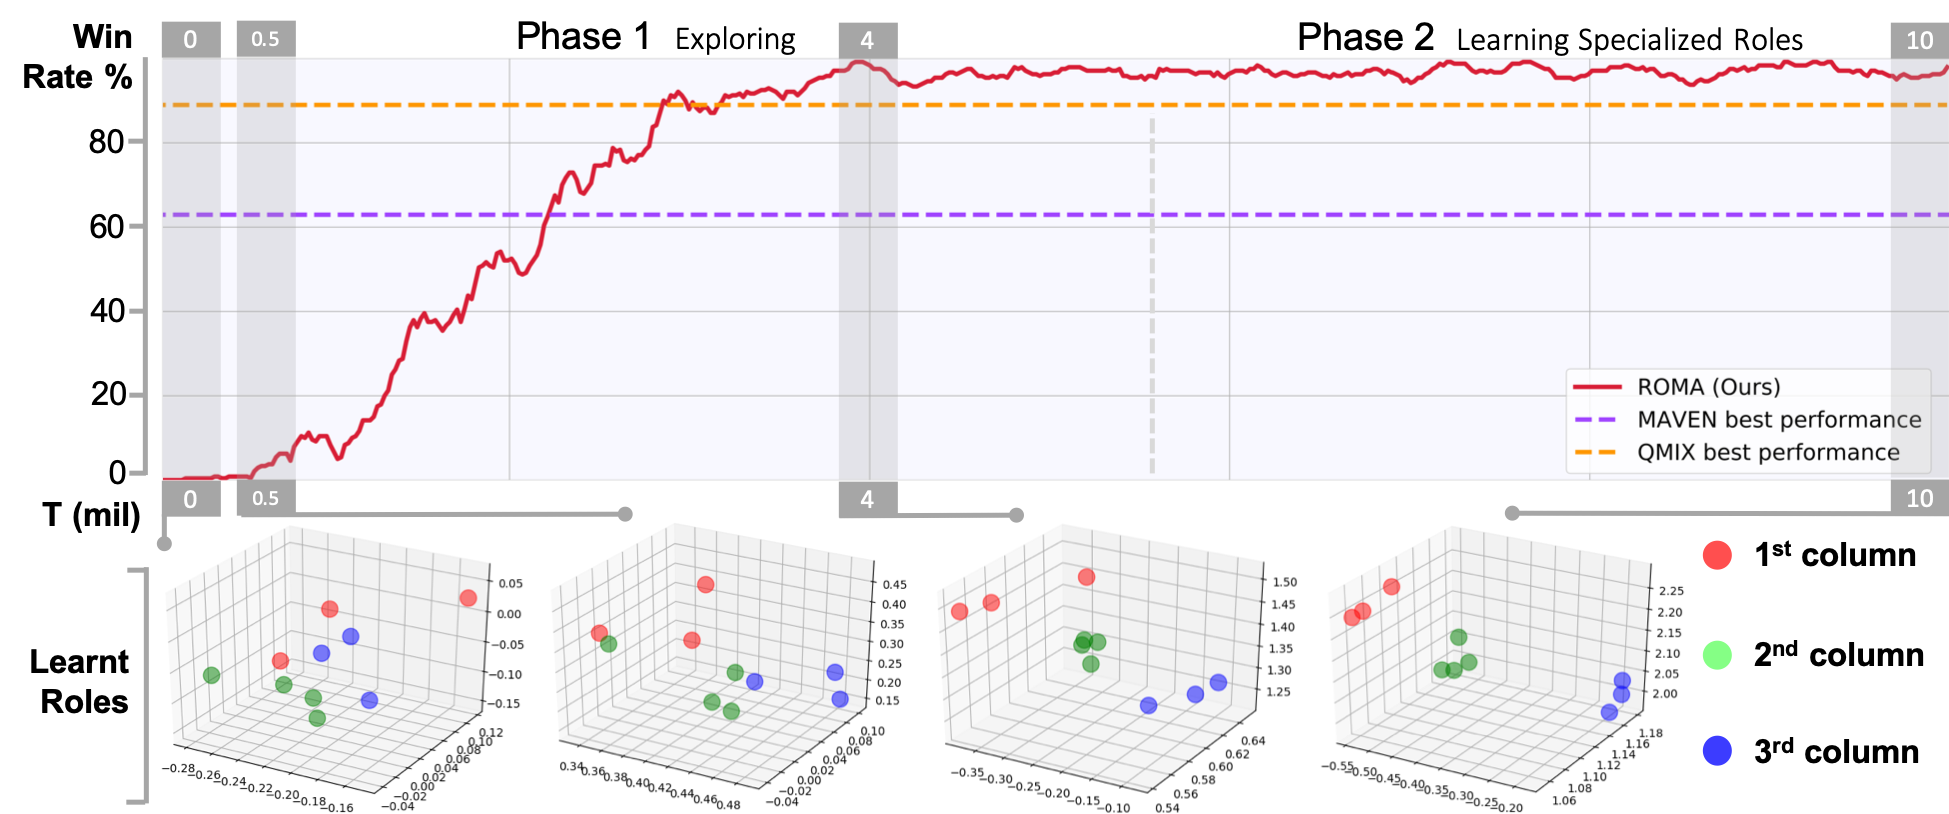
\includegraphics[width=\linewidth]{figures/evolution/evolution_10m_vs_11m.png}
  \caption{角色在$\mathtt{10m\_vs\_11m}$中的演化与涌现}\label{fig:role_evolution-homo}
\end{figure*}

在图~\ref{fig:role_evolution-homo}中同样可视化一个训练的胜率曲线和角色表征。这里展示的是同质环境$\mathtt{10m\_vs\_11m}$, 具体来说,我方有10个Marines, 敌方有11个Marines.

这里展示的是每一局最开始的角色的表征,胜利的策略是快速形成一个凹型的曲线阵列,已获得最大的射击范围(因为距离太远攻击不到). 可以清楚地看到,本算法逐渐学会根据智能体的相对位置来确定角色,这样的角色以及相对应的策略能够让整个集体快速完成站位,并且不发生冲突,这一点对胜利是很有必要的。正因为如此,可以联合胜率曲线和角色表征看到,随着角色的表征逐渐清晰,胜率也逐渐上升。

\subsection{小结}
从上面的异质和同质环境的角色演化和涌现可以发现,角色的涌现、演化并逐渐清晰,和胜率是密切相关的。

\section{实验配置细节}\label{sec:exp-detail}
局部效用函数由一层全连接FC, 一个64bit的GRU以及一层全连接组成,输入是观测,输出是对每个动作的Q值,这些Q值会进入到一个混合网络,这部分激活函数是ReLU。这些设置和QMIX完全一致。

本项目中的角色编码器、角色解码器、轨迹编码器都是两层的全连接网络,激活函数使用LeakyReLU. 所有的角色维数为3, 在可视化时候,没有使用降维。

超参设置为$\lambda_I=10^{-4}$, $\lambda_D=10^{-2}$, $\gamma=0.99$. 优化算法使用RMSprop, 学习率为$5\times 10^{-4}$. 强化学习的探索使用$\epsilon$-greedy, 其中$\epsilon$线性地在$50k$步内从$1.0$降到$0.05$. 

实验在NVIDIA GTX 2080 Ti GPU执行。

\section{本章小结}

本章进行了多种实验,从各个方面说明了本算法的有效和高效。

基准实验说明了本算法能够在性能上超越文献中的算法;消融实验说明了损失函数的有效性以及不同损失函数的作用;角色的动态变化图说明了本算法学到的角色能在适应环境过程中不断演化;角色的表征分析说明了角色与策略的对应关系;角色的演化与涌现说明了角色的逐渐演化对胜率有密切的影响。